\documentclass[11pt,a4paper]{article}

\usepackage[a4paper,margin=1in]{geometry}
\usepackage{graphicx}
\usepackage{booktabs}
\usepackage{amsmath,amssymb}
\usepackage{float}
\usepackage{hyperref}
\usepackage{xcolor}
\usepackage{enumitem}
\usepackage{fancyhdr}
\usepackage{longtable}

\hypersetup{colorlinks=true,linkcolor=blue,urlcolor=blue}

\pagestyle{fancy}
\fancyhf{}
\setlength{\headheight}{14pt}
\lhead{ICS1512}
\rhead{Machine Learning Algorithms Laboratory}
\cfoot{\thepage}
\renewcommand{\headrulewidth}{0.4pt}

\setlength{\parskip}{4pt}
\setlength{\parindent}{0pt}

\begin{document}

% ============================================================
% TITLE / STUDENT DETAILS
% ============================================================
\begin{center}
{\Large\bfseries Experiment 6: Bagging, Boosting, and Stacked Ensemble Models}
\end{center}
\vspace{4pt}

\begin{tabular}{|p{4cm}|p{11cm}|}
\hline
Experiment No. & 6 \\ \hline
Experiment Title & Bagging, Boosting, and Stacked Ensemble Models \\ \hline
Student Name & Sathiya Priyan \\ \hline
Register Number & 3122247001058 \\ \hline
Faculty & Dr. Poreddy Ajay Kumar Reddy \\ \hline
Submission Date & August 30, 2026 \\ \hline
\end{tabular}

\vspace{6pt}

% ============================================================
% OBJECTIVE
% ============================================================
\section{Objective}
To implement and compare three ensemble learning strategies -- Bagging (Decision Tree base learner),
Boosting (AdaBoost and Gradient Boosting), and a heterogeneous Stacked Ensemble (SVM, Naive Bayes,
Decision Tree with Logistic Regression as the meta learner) -- on the Wisconsin Diagnostic Breast
Cancer (WDBC) dataset, using 5-fold cross-validation for hyperparameter tuning and standard
classification metrics for final evaluation.

% ============================================================
% PROBLEM STATEMENT
% ============================================================
\section{Problem Statement}
\textbf{Input:} 30 numerical features derived from digitized FNA images of breast masses.
\textbf{Output:} Binary label -- \textbf{Malignant (M = 1)} or \textbf{Benign (B = 0)}.
\textbf{Task:} Supervised binary classification, solved using three ensemble strategies:

\begin{itemize}[nosep]
    \item \textbf{Bagging} -- multiple Decision Trees trained on bootstrap samples, combined by majority vote.
    \item \textbf{Boosting} -- AdaBoost and Gradient Boosting, trained sequentially to correct prior errors.
    \item \textbf{Stacking} -- SVM, Naive Bayes, and Decision Tree as base learners; Logistic Regression as meta learner.
\end{itemize}

% ============================================================
% DATASET DESCRIPTION
% ============================================================
\section{Dataset Description}
\begin{longtable}{|p{6cm}|p{8cm}|}
\hline
Dataset Name & Wisconsin Diagnostic Breast Cancer (WDBC) \\ \hline
Source & UCI ML Repository / \texttt{sklearn.datasets.load\_breast\_cancer} \\ \hline
Samples & 569 \\ \hline
Features & 30 numerical features \\ \hline
Classes & Benign = 357, Malignant = 212 \\ \hline
Train / Test Split & 455 / 114 (80\% / 20\%), \texttt{random\_state=42}, \texttt{stratify=y} \\ \hline
Missing Values & None (0 found) \\ \hline
\end{longtable}

\begin{figure}[H]
\centering
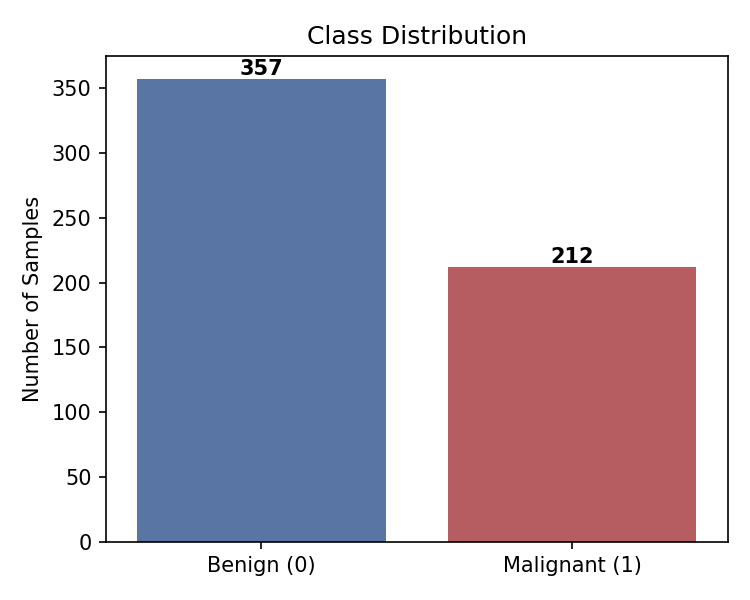
\includegraphics[width=0.55\linewidth]{figures/class_distribution_exp7.png}
\caption{Class distribution: 357 Benign vs. 212 Malignant samples.}
\end{figure}

The classes are moderately imbalanced ($\approx$63\% Benign, 37\% Malignant), so stratified sampling
was used for the train-test split and for cross-validation folds.

\begin{figure}[H]
\centering
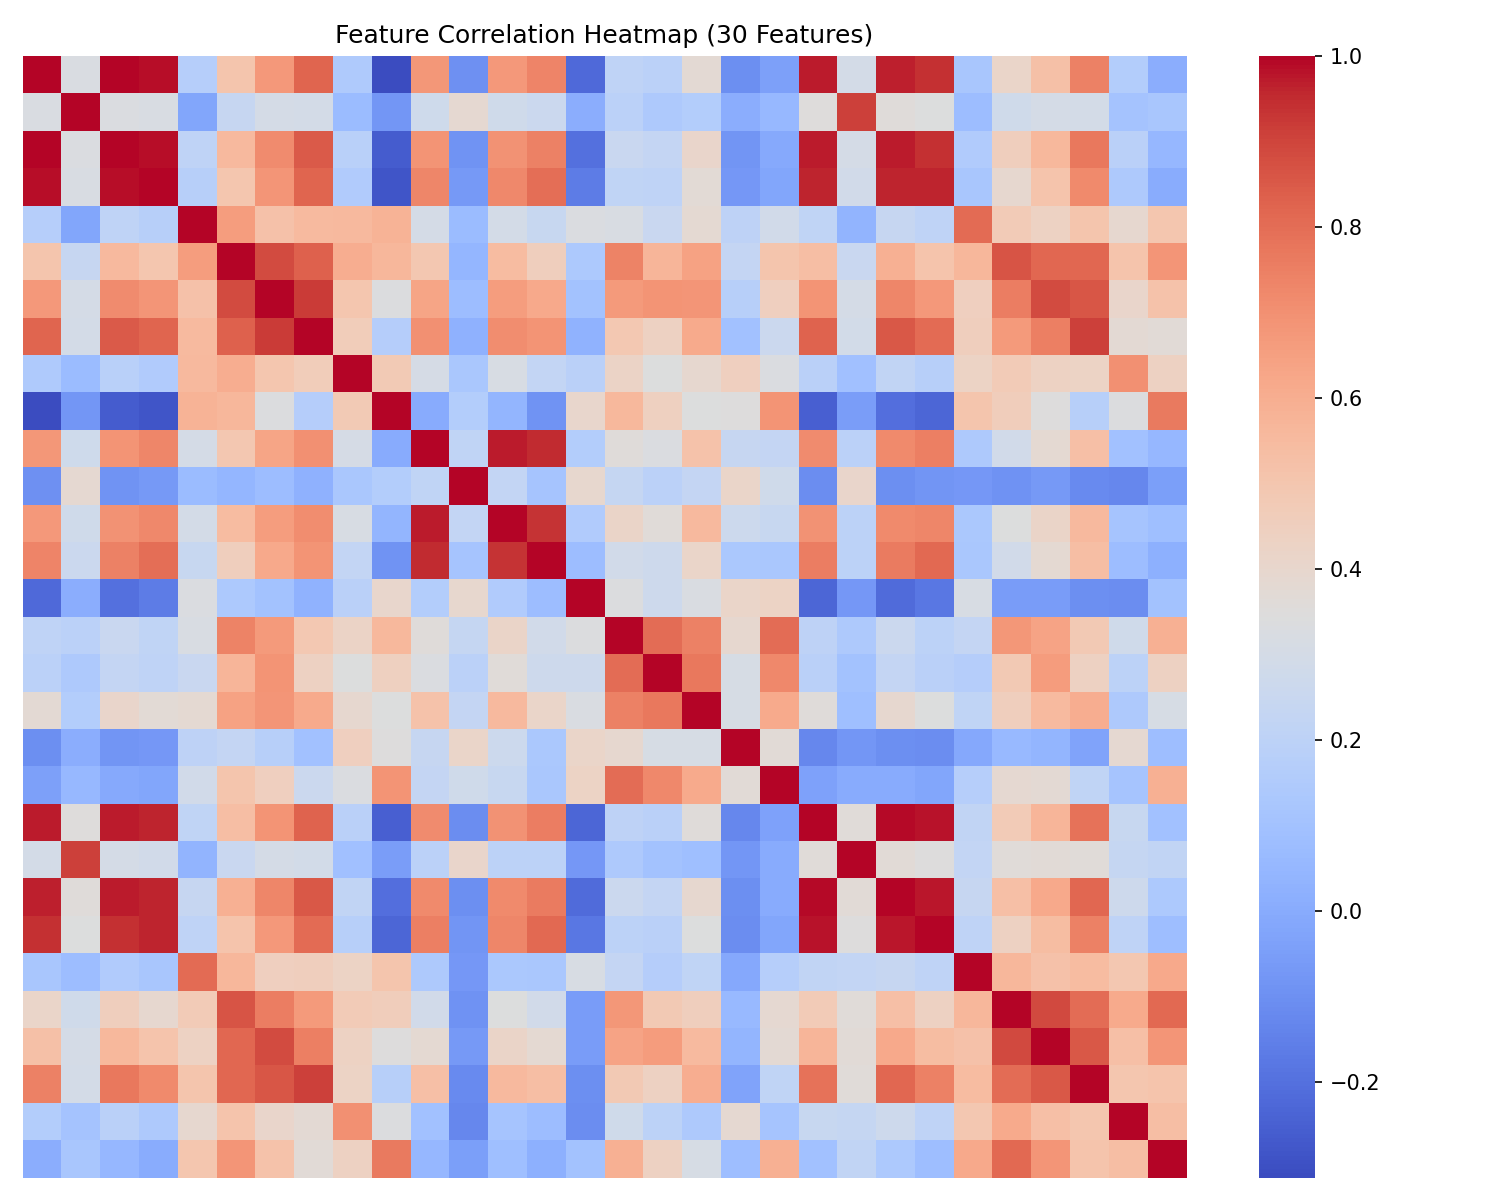
\includegraphics[width=0.6\linewidth]{figures/correlation_exp7.png}
\caption{Correlation heatmap of the 30 WDBC features.}
\end{figure}

Several radius-, perimeter-, and area-based features are strongly correlated, as expected since they
describe related geometric properties of the same cell nuclei.

% ============================================================
% PREPROCESSING
% ============================================================
\section{Data Preprocessing}
\begin{itemize}[nosep]
    \item Checked for missing values -- none found.
    \item Target encoded as B $\rightarrow$ 0, M $\rightarrow$ 1.
    \item 80/20 stratified train-test split (\texttt{random\_state=42}).
    \item Features standardized with \texttt{StandardScaler} (fit on train only) for the SVM base learner in Stacking; tree-based models used raw features.
\end{itemize}

% ============================================================
% ALGORITHMS
% ============================================================
\section{Machine Learning Algorithms}

\subsection{Bagging}
Bootstrap Aggregation trains multiple Decision Trees independently on bootstrap resamples of the
training data; predictions are combined by majority vote. Tuned over
\texttt{n\_estimators} $\in\{10,50,100\}$, \texttt{max\_samples} $\in\{0.5,0.8,1.0\}$,
\texttt{max\_features} $\in\{0.5,0.8,1.0\}$. Bagging primarily reduces variance.

\subsection{Boosting}
AdaBoost and Gradient Boosting were both tuned; the better model by CV F1-score was selected for
final comparison. Search space: \texttt{n\_estimators} $\in\{50,100,150\}$,
\texttt{learning\_rate} $\in\{0.01,0.1,1.0\}$ (Gradient Boosting also over \texttt{max\_depth}
$\in\{1,3,5\}$). Boosting primarily reduces bias.

\subsection{Stacked Ensemble}
\begin{verbatim}
                 Training Data
          +-----------+-----------+
          |           |           |
         SVM      Naive Bayes   Decision Tree
          |           |           |
          +-----------+-----------+
                      |
              Logistic Regression (meta learner)
                      |
                Final Prediction
\end{verbatim}
Base learners were combined via 5-fold internal stacking CV; the meta learner (Logistic Regression)
learns how to weight the three base predictions.

% ============================================================
% HYPERPARAMETER SELECTION
% ============================================================
\section{Hyperparameter Selection (5-Fold CV)}

\begin{table}[H]
\centering
\caption{Best Configuration per Model (GridSearchCV, scoring = F1)}
\begin{tabular}{lll}
\toprule
Model & Best Hyperparameters & CV F1-score \\
\midrule
Bagging & n\_estimators=50, max\_samples=1.0, max\_features=0.5 & 0.958 \\
AdaBoost & n\_estimators=150, learning\_rate=1.0 & 0.961 \\
Gradient Boosting & n\_estimators=150, learning\_rate=1.0, max\_depth=1 & \textbf{0.967} \\
Stacking (SVM+NB+DT $\to$ LR) & default base learners, 5-fold internal CV & 0.964 \\
\bottomrule
\end{tabular}
\end{table}

Gradient Boosting outperformed AdaBoost on cross-validation F1-score (0.967 vs. 0.961) and was
therefore selected as the representative Boosting model for final test-set evaluation.

% ============================================================
% RESULTS
% ============================================================
\section{Results}

\begin{table}[H]
\centering
\caption{Final Test-Set Performance (114 held-out samples)}
\begin{tabular}{lccccc}
\toprule
Model & Accuracy & Precision & Recall & F1-score & ROC-AUC \\
\midrule
Bagging            & 0.965 & 1.000 & 0.905 & 0.950 & 0.995 \\
Boosting (GB)       & 0.965 & 1.000 & 0.905 & 0.950 & 0.988 \\
Stacked Ensemble    & \textbf{0.974} & 1.000 & \textbf{0.929} & \textbf{0.963} & \textbf{0.997} \\
\bottomrule
\end{tabular}
\end{table}

All three models achieved perfect precision on the test set (no benign sample was misclassified as
malignant), and the Stacked Ensemble achieved the highest recall, F1-score, accuracy, and AUC.

% ============================================================
% VISUALIZATION
% ============================================================
\section{Result Visualization}

\begin{figure}[H]
\centering
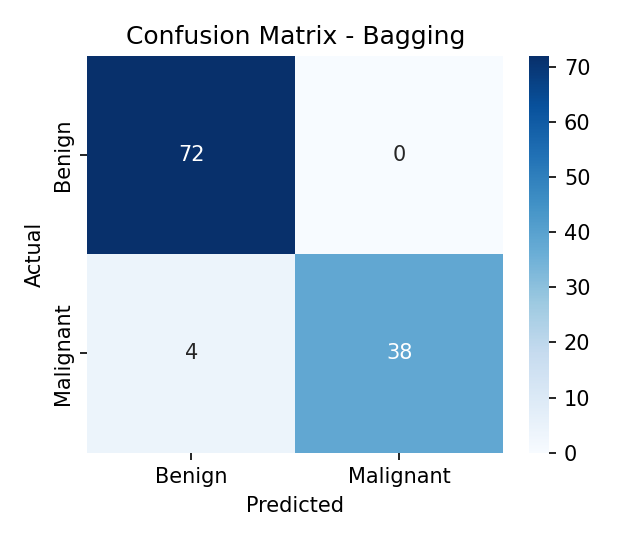
\includegraphics[width=0.4\linewidth]{figures/cm_bagging_exp7.png}\hfill
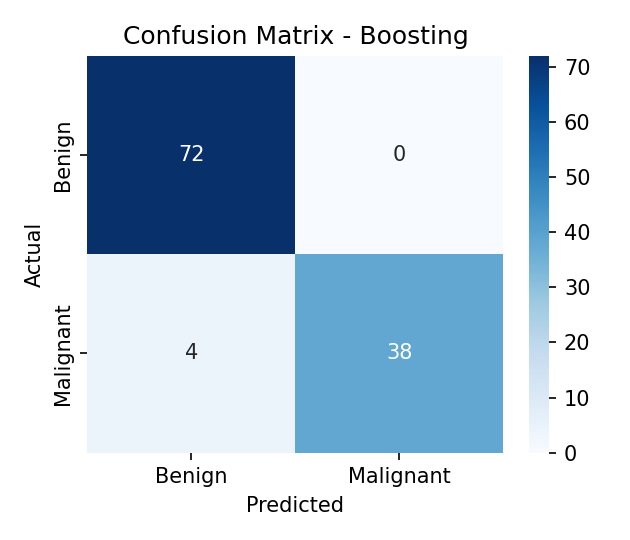
\includegraphics[width=0.4\linewidth]{figures/cm_boosting_exp7.png}
\caption{Confusion matrices -- Bagging (left) and Boosting (right). Both misclassify 4 malignant cases as benign.}
\end{figure}

\begin{figure}[H]
\centering
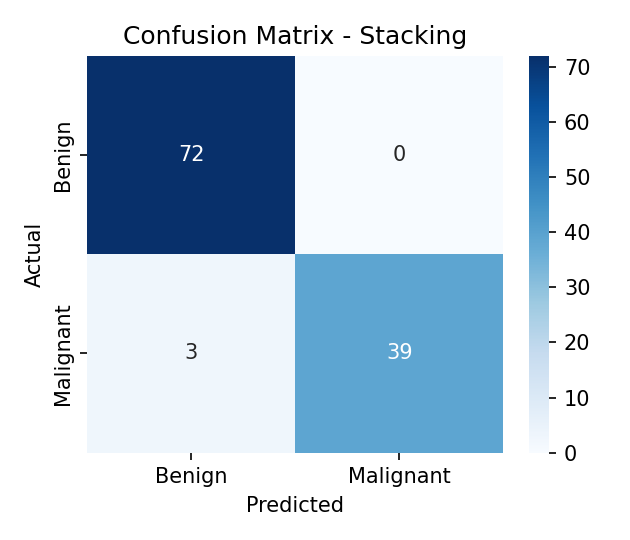
\includegraphics[width=0.4\linewidth]{figures/cm_stacking_exp7.png}
\caption{Confusion matrix -- Stacked Ensemble. Only 3 malignant cases misclassified as benign, the fewest of all models.}
\end{figure}

\begin{figure}[H]
\centering
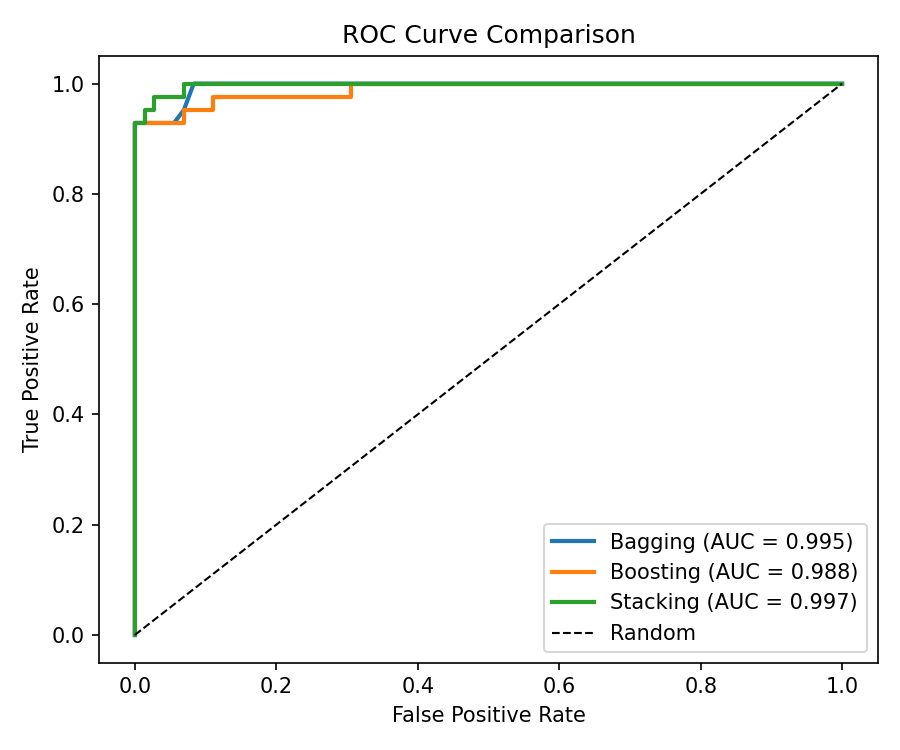
\includegraphics[width=0.65\linewidth]{figures/roc_comparison_exp7.png}
\caption{ROC curve comparison. The Stacked Ensemble (AUC = 0.997) dominates Bagging (AUC = 0.995) and Boosting (AUC = 0.988) across nearly all thresholds.}
\end{figure}

% ============================================================
% DISCUSSION
% ============================================================
\section{Discussion}

\textbf{Bias-variance perspective:} Bagging reduces variance by averaging many independently trained
Decision Trees over bootstrap samples, stabilizing predictions that would otherwise be sensitive to
the specific training subset. Boosting instead reduces bias by sequentially fitting learners to the
residual errors of previous rounds -- Gradient Boosting's shallow (\texttt{max\_depth=1}) trees with
\texttt{learning\_rate=1.0} converged to the best CV F1-score among boosting variants. Stacking
benefits from combining heterogeneous inductive biases: SVM's margin-based boundary, Naive Bayes'
probabilistic independence assumption, and the Decision Tree's axis-aligned splits each capture
different structure in the data, and the Logistic Regression meta learner learns to weight these
complementary signals.

\textbf{Generalization:} Cross-validation and test performance are close for all three models
(e.g., Stacking: CV F1 = 0.964 vs. test F1 = 0.963), indicating good generalization with minimal
overfitting.

% ============================================================
% OBSERVATION QUESTIONS
% ============================================================
\section{Observation Questions}

\textbf{How does Bagging reduce variance?}
By training multiple Decision Trees on independent bootstrap samples and aggregating via majority
vote, individual trees' overfitting tendencies are averaged out, producing a more stable classifier.

\textbf{How does Boosting address model bias?}
Boosting fits learners sequentially, with each new learner focusing on the errors of the ensemble so
far; this iterative error-correction reduces systematic bias that a single weak learner would retain.

\textbf{Why does Stacking benefit from heterogeneous models?}
SVM, Naive Bayes, and Decision Tree make different structural assumptions about the data, so their
errors are only partially correlated. The meta learner exploits this by learning an optimal
combination, which is why Stacking achieved the best overall test-set F1-score (0.963) in this
experiment.

\textbf{Which ensemble method performed best and why?}
The \textbf{Stacked Ensemble} performed best (Accuracy = 0.974, F1 = 0.963, AUC = 0.997), because
combining heterogeneous base learners captured complementary decision boundaries that neither
Bagging (variance reduction alone) nor Boosting (bias reduction alone) could match individually.

% ============================================================
% CONCLUSION
% ============================================================
\section{Conclusion}
Bagging, Boosting (AdaBoost / Gradient Boosting), and a Stacked Ensemble (SVM + Naive Bayes +
Decision Tree with a Logistic Regression meta learner) were implemented and tuned via 5-fold
cross-validation on the WDBC dataset. On the held-out test set, all models exceeded 96\% accuracy
and 0.98 AUC, with the Stacked Ensemble achieving the best overall performance
(Accuracy = 97.4\%, F1 = 0.963, AUC = 0.997), confirming that combining heterogeneous base learners
can outperform single-family ensembles for this classification task.

% ============================================================
% REFERENCES
% ============================================================
\section{References}
\small
\begin{enumerate}[label={[\arabic*]}]
\item scikit-learn developers, ``Ensemble Methods,'' \url{https://scikit-learn.org/stable/modules/ensemble.html}
\item scikit-learn developers, ``BaggingClassifier,'' \url{https://scikit-learn.org/stable/modules/generated/sklearn.ensemble.BaggingClassifier.html}
\item scikit-learn developers, ``AdaBoostClassifier,'' \url{https://scikit-learn.org/stable/modules/generated/sklearn.ensemble.AdaBoostClassifier.html}
\item scikit-learn developers, ``StackingClassifier,'' \url{https://scikit-learn.org/stable/modules/generated/sklearn.ensemble.StackingClassifier.html}
\item UCI Machine Learning Repository, ``Breast Cancer Wisconsin (Diagnostic) Dataset,'' \url{https://archive.ics.uci.edu}
\end{enumerate}

\end{document}
